\documentclass[../../main.tex]{subfiles}

\begin{document}

Mittlerweile hast du eine ganze Reihe von Beispielen für Mengen gesehen -- und damit auch eine ganze Reihe von Dingen, die Elemente einer Menge sein können: Farben, Tierarten, Buchstaben, Zahlen usw.

Weil wir Mengen meist als Oberbegriff für bestimmte Dinge verwendet haben (zum Beispiel $\Natural$ als Oberbegriff für die Zahlen $1,2,3,\dots$), haben wir uns immer nur dafür interessiert, welche Dinge Elemente der Menge sind und welche nicht. Wir haben uns nicht um eine Reihenfolge oder dergleichen gekümmert: Die Mengen $\{4,1\}$ und $\{1,4\}$ sind gleich, da sie beide dieselben Elemente enthalten -- und es ist egal, in welcher Reihenfolge wir sie aufschreiben. Bei Mengen gibt es also nie eine Information über die Reihenfolge, in der ihre Elemente vorkommen. 

Aufbauend auf dem Wissen, dass du Dinge mithilfe von Mengen zu Oberbegriffen zusammenfassen kannst, lernst du in diesem Abschnitt, wie sich verschiedene Objekte (z.B. Zahlen, Gegenstände) sogar noch strukturierter zusammenfassen lassen. Auch in den nächsten Kapiteln wirst du feststellen, dass mithilfe von Mengen und Begriffen, die auf ihnen aufbauen, sehr viele Zusammenhänge aus dem Leben erfasst werden können.

\begin{example}[ex:fussball-tupel]{}
    \parpic[r]{
        
\includegraphics[height=2.8cm]{images/fussball.pdf}
    }
    Das Ergebnis eines Fußballspiels zwischen dem FC Bayern München und Borussia Dortmund, das mit $3:2$ für Bayern entschieden worden ist, enthält zwei Zahlen, nämlich die $3$ und die $2$. Wir haben zwei Informationen, nämlich die Anzahl der Heimtore und die Anzahl der Auswärtstore.
    
    \picskip{2}
    Üblicherweise redest du über das Ergebnis des Spiels, ohne darüber nachzudenken, dass es aus zwei separaten Informationen besteht. Es wäre natürlich schön, wenn es uns gelingen würde, das mathematisch zu repräsentieren. Denn erstmal haben wir nur zwei einzelne Zahlen, $2$ und $3$. Wenn wenn wir das Ergebnis in der Menge $\{3,2\}$ zusammenfassen, dann geht die Information verloren, welches der beiden Teams $3$ Tore geschossen hat und welches nur $2$, denn die Mengen $\{3,2\}$ und $\{2,3\}$ sind gleich. Diese Menge wäre ein Oberbegriff für die Zahlen $2$ und $3$, aber keine Beschreibung dafür, \emph{welche} Mannschaft $2$ und welche $3$ Tore geschossen hat.
\end{example}

\parpic[r]{
    \begin{tikzpicture}
        \node at (0,0) {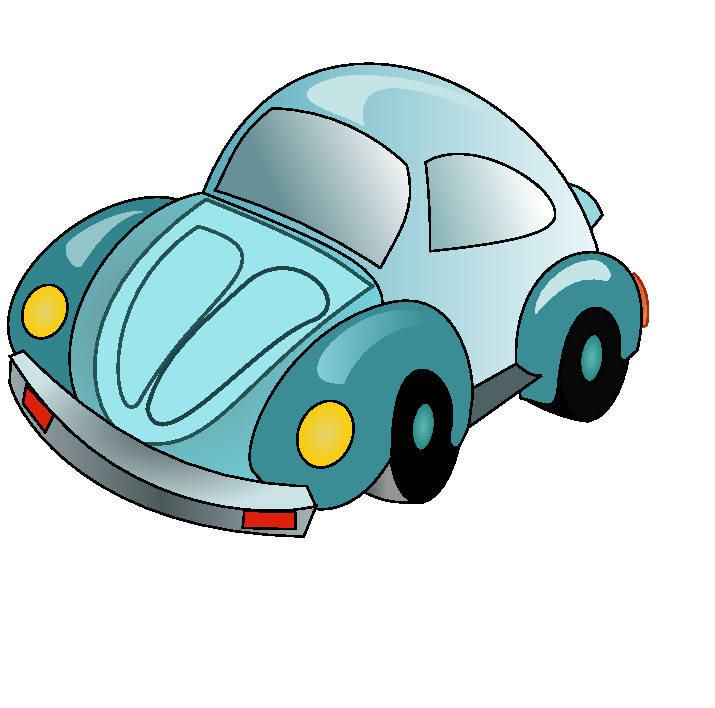
\includegraphics[width=.25\textwidth]{images/car.pdf}};
        \draw[fill=maincolor,maincolor] (-0.1,1.3) -- (-0.6,1.6) circle[radius=.6mm] node[above] {\small Farbe};
        \draw[fill=maincolor,maincolor] (0.8,-0.1) -- (0.6,-0.8) circle[radius=.6mm] node[below] {\small Automarke};
        \draw[fill=maincolor,maincolor] (-1,-0.3) -- (-1.4,-1.1) circle[radius=.6mm] node[below] {\small PS};
    \end{tikzpicture}
}

Im letzten Beispiel haben wir mehrere Informationen gesehen, die wir zusammenfassen wollen. Es lassen sich viele weitere Beispiele finden, in denen ein großes Ganzes aus mehreren kleineren \textbf{Komponenten} besteht: Das Ergebnis eines Fußballspiels besteht aus den Heim- und den Auswärtstoren. Zu den Eigenschaften eines Autos gehören seine Marke, seine Farbe und seine Pferdestärke. Ein Malset besteht aus Pinseln, Farben und weiteren Utensilien. Ein Buch hat einen Autor, einen Titel, Hauptcharaktere und vieles mehr.

\parpic[r]{
    \begin{tikzpicture}
        \fill[grayset] (0,0.5) -- (2,0.5) -- (2,0.5) arc (90:-90:0.5) -- (2,-0.5) -- (0,-0.5) -- (0,-0.5) arc (270:90:0.5) -- cycle;
        \foreach \x in {0.5,1.5}{
            \fill[black!25!white] (\x,0) circle[radius=0.25];
            \draw[line width=0.025cm] (\x,0) circle[radius=0.25];
        }
        \node[maincolor] at (1,0.75) {Komponenten};
        \node at (1,-0.75) {\small \textbf{Tupel}};
        \draw[maincolor,->] (0.5,0.55) -- (0.5,0.25);
        \draw[maincolor,->] (1.5,0.55) -- (1.5,0.25);
    \end{tikzpicture}
}

\picskip{5}
In all diesen Beispielen gibt es also eine Sache, die, wenn wir genauer hinschauen, viele verschiedene Details und Eigenschaften hat. Solche Eigenschaften würden wir gern so zusammenfassen, dass sie mathematisch durch ein einzelnes Objekt beschrieben werden können. Das Mittel der Wahl dafür sind \textbf{Tupel}. Du kannst dir ein Tupel als eine Art Stecksystem vorstellen (wie im Bild rechts), zu dem verschiedene Komponenten gehören, die seine Eigenschaften beschreiben. Ein Tupel fasst also mehrere \textbf{Komponenten} zu einem großen Ganzen zusammen.

Mathematisch sind diese Eigenschaften einfach eine Liste von Informationen -- ähnlich wie bei einer Menge. Der Unterschied ist, dass jede Information nun zu einem bestimmten Steckplatz gehört. Dadurch sind sie geordnet. Aufgeschrieben wird ein solches Tupel mit den Komponenten $x_1,x_2,\dots,x_n$ in runden Klammern
\[(x_1,x_2,\dots,x_n),\]
damit es von einer Menge unterschieden werden kann, die ja in geschweiften Klammern geschrieben wird.

\begin{example}{}
    \parpic[r]{
        \begin{tikzpicture}
            \fill[grayset] (0,0.5) -- (2,0.5) -- (2,0.5) arc (90:-90:0.5) -- (2,-0.5) -- (0,-0.5) -- (0,-0.5) arc (270:90:0.5) -- cycle;
            \foreach \x in {0.5,1.5}{
                \fill[black!25!white] (\x,0) circle[radius=0.25];
                \draw[line width=0.025cm] (\x,0) circle[radius=0.25];
            }
            \node[maincolor] at (0.5,0.75) {Heimtore};
            \draw[maincolor,->] (0.5,0.55) -- (0.5,0.25);
            \draw[maincolor,->] (1.5,-0.55) -- (1.5,-0.25);
            \node[maincolor] at (1.5,-0.75) {Auswärtstore};
            \node at (0.5,0) {$3$};
            \node at (1.5,0) {$2$};
        \end{tikzpicture}
    }
    Das Ergebnis des Fußballspiels aus Beispiel \ref{ex:fussball-tupel} besteht aus zwei Komponenten: Der Anzahl der Heimtore und der Anzahl der Auswärtstore. Auf der Ergebnisanzeige würden diese beiden Informationen einfach nebeneinander angezeigt werden, etwa so wie auf der rechten Seite. 
    
    \picskip{0}
    Die beiden Komponenten des Ergebnisses können wir nebeneinander auf das rechts abgebildete Stecksystem stecken. Das, was wir links hin stecken, ist die Anzahl der Heimtore und das, was wir rechts hin stecken, ist die Anzahl der Auswärtstore. Für das $3:2$ aus unserem Beispiel können wir dieses Stecksystem als $(3,2)$ notieren.
\end{example}

\begin{example}{}
    Die Schulleitung hatte mal wieder ein neues Auto nötig und hat ein Auto wie das rechts auf der letzten Seite abgebildete hellblaue Auto der Marke \emph{Faul-Drive} erworben. Der Hersteller verspricht eine Motorleistung von $75\,\text{PS}$.

    Diese drei \emph{Komponenten} beschreiben zusammen (zumindest einige) Eigenschaften des neuen Autos. Wenn wir das Auto nun als ein einziges mathematisches Objekt darstellen möchten, das diese drei Informationen enthält, dann können wir die Eigenschaften zu einem Tupel zusammenfassen:
    \[\textsc{Auto}=(\text{hellblau}, \text{Faul-Drive}, 75\,\text{PS})\]
    Die erste Komponente ist die Farbe des Autos, die zweite Komponente die Marke und die dritte die Pferdestärke.
\end{example}

Da Tupel eine Art Steckvorrichtung sind, haben sie immer eine bestimmte Anzahl von Komponenten. Zur Ergebnisdarstellung benötigen wir zwei Komponenten, für Autos sind wir mit drei Komponenten ausgekommen. Abhängig von der Anzahl $n$ seiner Komponenten wird ein $n$-Tupel allgemein wie folgt definiert.

\begin{definition}{Tupel}
    Ein \textbf{\emph{n}-Tupel} ist eine \textit{geordnete} Liste von $n$ Objekten. Wir schreiben für ein $n$-Tupel mit den Objekten $x_1,\dots,x_n$:
    \[(x_1,\dots,x_n)\]
    und nennen $x_1,\dots,x_n$ die \textbf{Komponenten} des Tupels.
\end{definition}

Auch wenn Tupel für dich noch ein relativ neues Konzept sind, hast du sie bereits deutlich früher in diesem Buch gesehen, nämlich, als du dich mit Koordinatensystemen beschäftigt hast. Ein Punkt im Koordinatensystem besteht immer aus zwei Informationen: Seiner $x$-Koordinate und seiner $y$-Koordinate.

\begin{example}{}
    Koordinaten
\end{example}

$2$-Tupel eignen sich also hervorragend, um Punkte in einem Koordinatensystem zu beschreiben. Da die Komponenten eines $2$-Tupels aber irgendwelche beliebigen Objekte sein können, eignet sich nicht jedes $2$-Tupel, um einen Punkt darzustellen:
\begin{multicols}{3}
    \[(4,11)\]

    \[(\text{Faultier},0)\]

    \[(\text{blau},-9)\]
\end{multicols}
Nur das linke dieser drei $2$-Tupel beschreibt sinnvoll einen Punkt, denn die Koordinaten eines Punktes sollten sinnvollerweise Zahlen sein. Für die Zahlen, die wir kennen, haben wir in Abschnitt \ref{chapter:zahlenmengen} einen Namen kennengelernt: Die reellen Zahlen \Real. Die Punkte eines Koordinatensystems sind also nicht irgendwelche $2$-Tupel, sondern nur solche, deren Komponenten beide aus \Real kommen. Mathematisch aufgeschrieben benötigen wir also Tupel $(x,y)$ mit der Eigenschaft, dass $x\in\Real$ und $y\in\Real$ gilt.

Weil wir mit Tupeln fast immer ganz bestimmte Dinge beschreiben wollen, ist es auch fast immer sinnvoll, im Vorfeld bereits festzulegen, aus welchen Wertebereichen die Komponenten kommen können. Für diese Wertebereiche kennen wir auch schon ein mathematisches Wort: \emph{Mengen}. Insgesamt interessieren wir uns also meistens für bestimmte Tupel, deren Komponenten jeweils aus bestimmten Mengen kommen.

\begin{example}{}
\end{example}

Die Tupel, die entstehen, wenn wir mehrere Mengen wie im letzten Beispiel kombinieren, sind Teil des \textbf{kartesischen Produkts} der Mengen. Dieses schreibt man auf, indem man zwischen die Mengen, die kombiniert werden sollen, das Zeichen $\times$ schreibt. Das kartesische Produkt der Mengen $M$ und $N$, das wir als 
\[M \times N\]
schreiben können, besteht aus allen Tupeln, deren erste Komponente aus $M$ und deren zweite Komponente aus $N$ gehört, also
\[M \times N=\{(m,n) \mid m\in N, n\in N\}.\]

\begin{definition}{Kartesisches Produkt}
    Das \textbf{kartesische Produkt} zweier Mengen $M$ und $N$ ist die Menge
    \[M\times N:=\{(m,n)~|~m\in M, n\in N\}\]
    aller $2$-Tupel $(m,n)$, deren erste Komponente aus $M$ und deren zweite Komponente aus $N$ kommt.
\end{definition}

\begin{example}{}
    Schach?
\end{example}

\begin{advanced}{Potenz einer Menge}
    Wenn wir das kartesische Produkt einer Menge mit sich selbst bilden -- ggf. auch sehr oft -- dann können wir, ähnlich wie bei der wiederholten Multiplikation eine Potenzschreibweise verwenden.

    \begin{definition}{Potenz einer Menge}
        Es sei $M$ eine Menge. Dann schreiben wir statt $\underbrace{M\times \dots\times M}_{n-\text{mal}}$ auch $M^n$.
    \end{definition}

    Die Punkte im Koordinatensystem können, wie du bereits weißt, mit Tupeln aus der menge $\Real\times\Real$ dargestellt werden. Oft werden die Punkte im Koordinatensystem als Elemente der Menge $\Real^2$ aufgefasst. Dadurch lassen sich auch Punkte in höherdimensionalen Koordinatensystemen beschreiben. Du wirst später ein 3D-Koordinatensystem kennenlernen, dessen Punkte Tupel aus $\Real^3$ sind. Tatsächlich ergibt es aber auch Sinn, mit noch viel höheren Dimensionen zu arbeiten. Das Rechnen mit Punkten der Menge $\Real^n$ für große $n\in\Natural$ ist beispielsweise eine wichtige Voraussetzung für moderne künstliche Intelligenz.
\end{advanced}

\begin{theorem}{}
    Das kartesische Produkt $M\times N$ zweier Mengen $M$ und $N$ mit $|M|=m$ und $|N|=n$ hat genau $m\cdot n$ Elemente.
\end{theorem}

\begin{nutshell}{Tupel und das kartesische Produkt}
    \parpic[r]{
        \begin{tikzpicture}
            \fill[grayset] (0,0.5) -- (2,0.5) -- (2,0.5) arc (90:-90:0.5) -- (2,-0.5) -- (0,-0.5) -- (0,-0.5) arc (270:90:0.5) -- cycle;
            \foreach \x in {0.5,1.5}{
                \fill[black!25!white] (\x,0) circle[radius=0.25];
                \draw[line width=0.025cm] (\x,0) circle[radius=0.25];
            }
            \node[maincolor] at (1,0.75) {Komponenten};
            \draw[maincolor,->] (0.5,0.55) -- (0.5,0.25);
            \draw[maincolor,->] (1.5,0.55) -- (1.5,0.25);
        \end{tikzpicture}
    }
    Bei einem \textbf{Tupel} werden mehrere Objekte oder Informationen \emph{geordnet} in einer Liste zusammengefasst. Die Einträge einer solchen Liste werden die \textbf{Komponenten} des Tupels genannt. Ein \textbf{\emph{n}-Tupel} ist eine Liste mit $n$ Komponenten $x_1,\dots,x_n$ und wird mit \[(x_1,\dots,x_n)\] 
    notiert. Im Gegensatz zu Mengen ist die Reihenfolge der Komponenten bei Tupeln relevant. Zwei Mengen $M$ und $N$ lassen sich mithilfe des \textbf{kartesischen Produkts} kombinieren, um die Menge 
    \[M\times N:=\{(m,n)~|~m\in M, n\in N\}\]
    zu erhalten, die aus Tupeln besteht, deren erste Komponente aus $M$ und deren zweite Komponente aus $N$ kommt.
\end{nutshell}

\end{document}